 % mainfile: ../../../../master.tex
\subsection{Understand Comprehensive Android Invocation Flow}
\label{task:20240121_aosp}

\subsubsection{System Server}

Startup process\footnote{\url{https://blog.csdn.net/q1210249579/article/details/128793307}}

ServiceManager vs SystemServiceManager \footnote{\url{https://blog.csdn.net/b1480521874/article/details/79422909}}

Looper\footnote{\url{https://stackoverflow.com/questions/35931899/why-main-threads-looper-loop-doesnt-block-ui-thread}} is at the end of System Server to pop messages from message queue and invoke the corresponding methods to handle it.`'

\subsubsection{System UI}

WindowManagerService\footnote{\url{https://blog.csdn.net/CallmeZhe/article/details/113989896}}

Loading of System UI \footnote{\url{https://stackoverflow.com/questions/37465026/when-systemui-loads-in-android-boot}}



\subsubsection{Activity Manager}

The Activity manager is started by Android's Zygote's System Services

Android application launch process\footnote{\url{https://multi-core-dump.blogspot.com/2010/04/android-application-launch.html}, \url{https://multi-core-dump.blogspot.com/2010/04/android-application-launch-part-2.html}, and \url{https://blog.csdn.net/u012481172/article/details/49658633}}

Role of ActivityManager\footnote{\url{https://developer.android.com/reference/android/app/ActivityManager\#nested-classes}}

Role\footnote{\url{https://blog.csdn.net/hzwailll/article/details/85339714}} of ActivityThread\footnote{\url{https://android.googlesource.com/platform/frameworks/base/+/master/core/java/android/app/ActivityThread.java}}

Role\footnote{\url{https://stackoverflow.com/questions/29140889/when-is-instrumentation-involved-in-app-start}} of Instrumentation\footnote{\url{https://developer.android.com/reference/android/app/Instrumentation}}

Activity Record\footnote{\url{https://stackoverflow.com/questions/18127984/what-is-activity-record-object-in-android}}

Tasks\footnote{\url{https://www.youtube.com/watch?v=MvIlVsXxXmY}}

Starting Activity\footnote{\url{https://duanqz.github.io/2016-07-29-Activity-LaunchProcess-Part1}}

Start Activty to Zygote Flow\footnote{\url[https://github.com/Marukohe/blog-notes/issues/4]}

\subsubsection{ART Invocation}

Method Execute Flow\footnote{\url{https://huanle19891345.github.io/en/android/art/jni/java_jni\%E6\%96\%B9\%E6\%B3\%95\%E8\%B0\%83\%E7\%94\%A8\%E5\%8E\%9F\%E7\%90\%86/}}

Dex2Oat\footnote{\url{https://huanle19891345.github.io/en/android/art/1\%E7\%B1\%BB\%E7\%BC\%96\%E8\%AF\%91/dex2oat/}}

\includepdf[pages=-, scale=.95,pagecommand={}]{entries/2024/01/21/Autism.pdf}

% 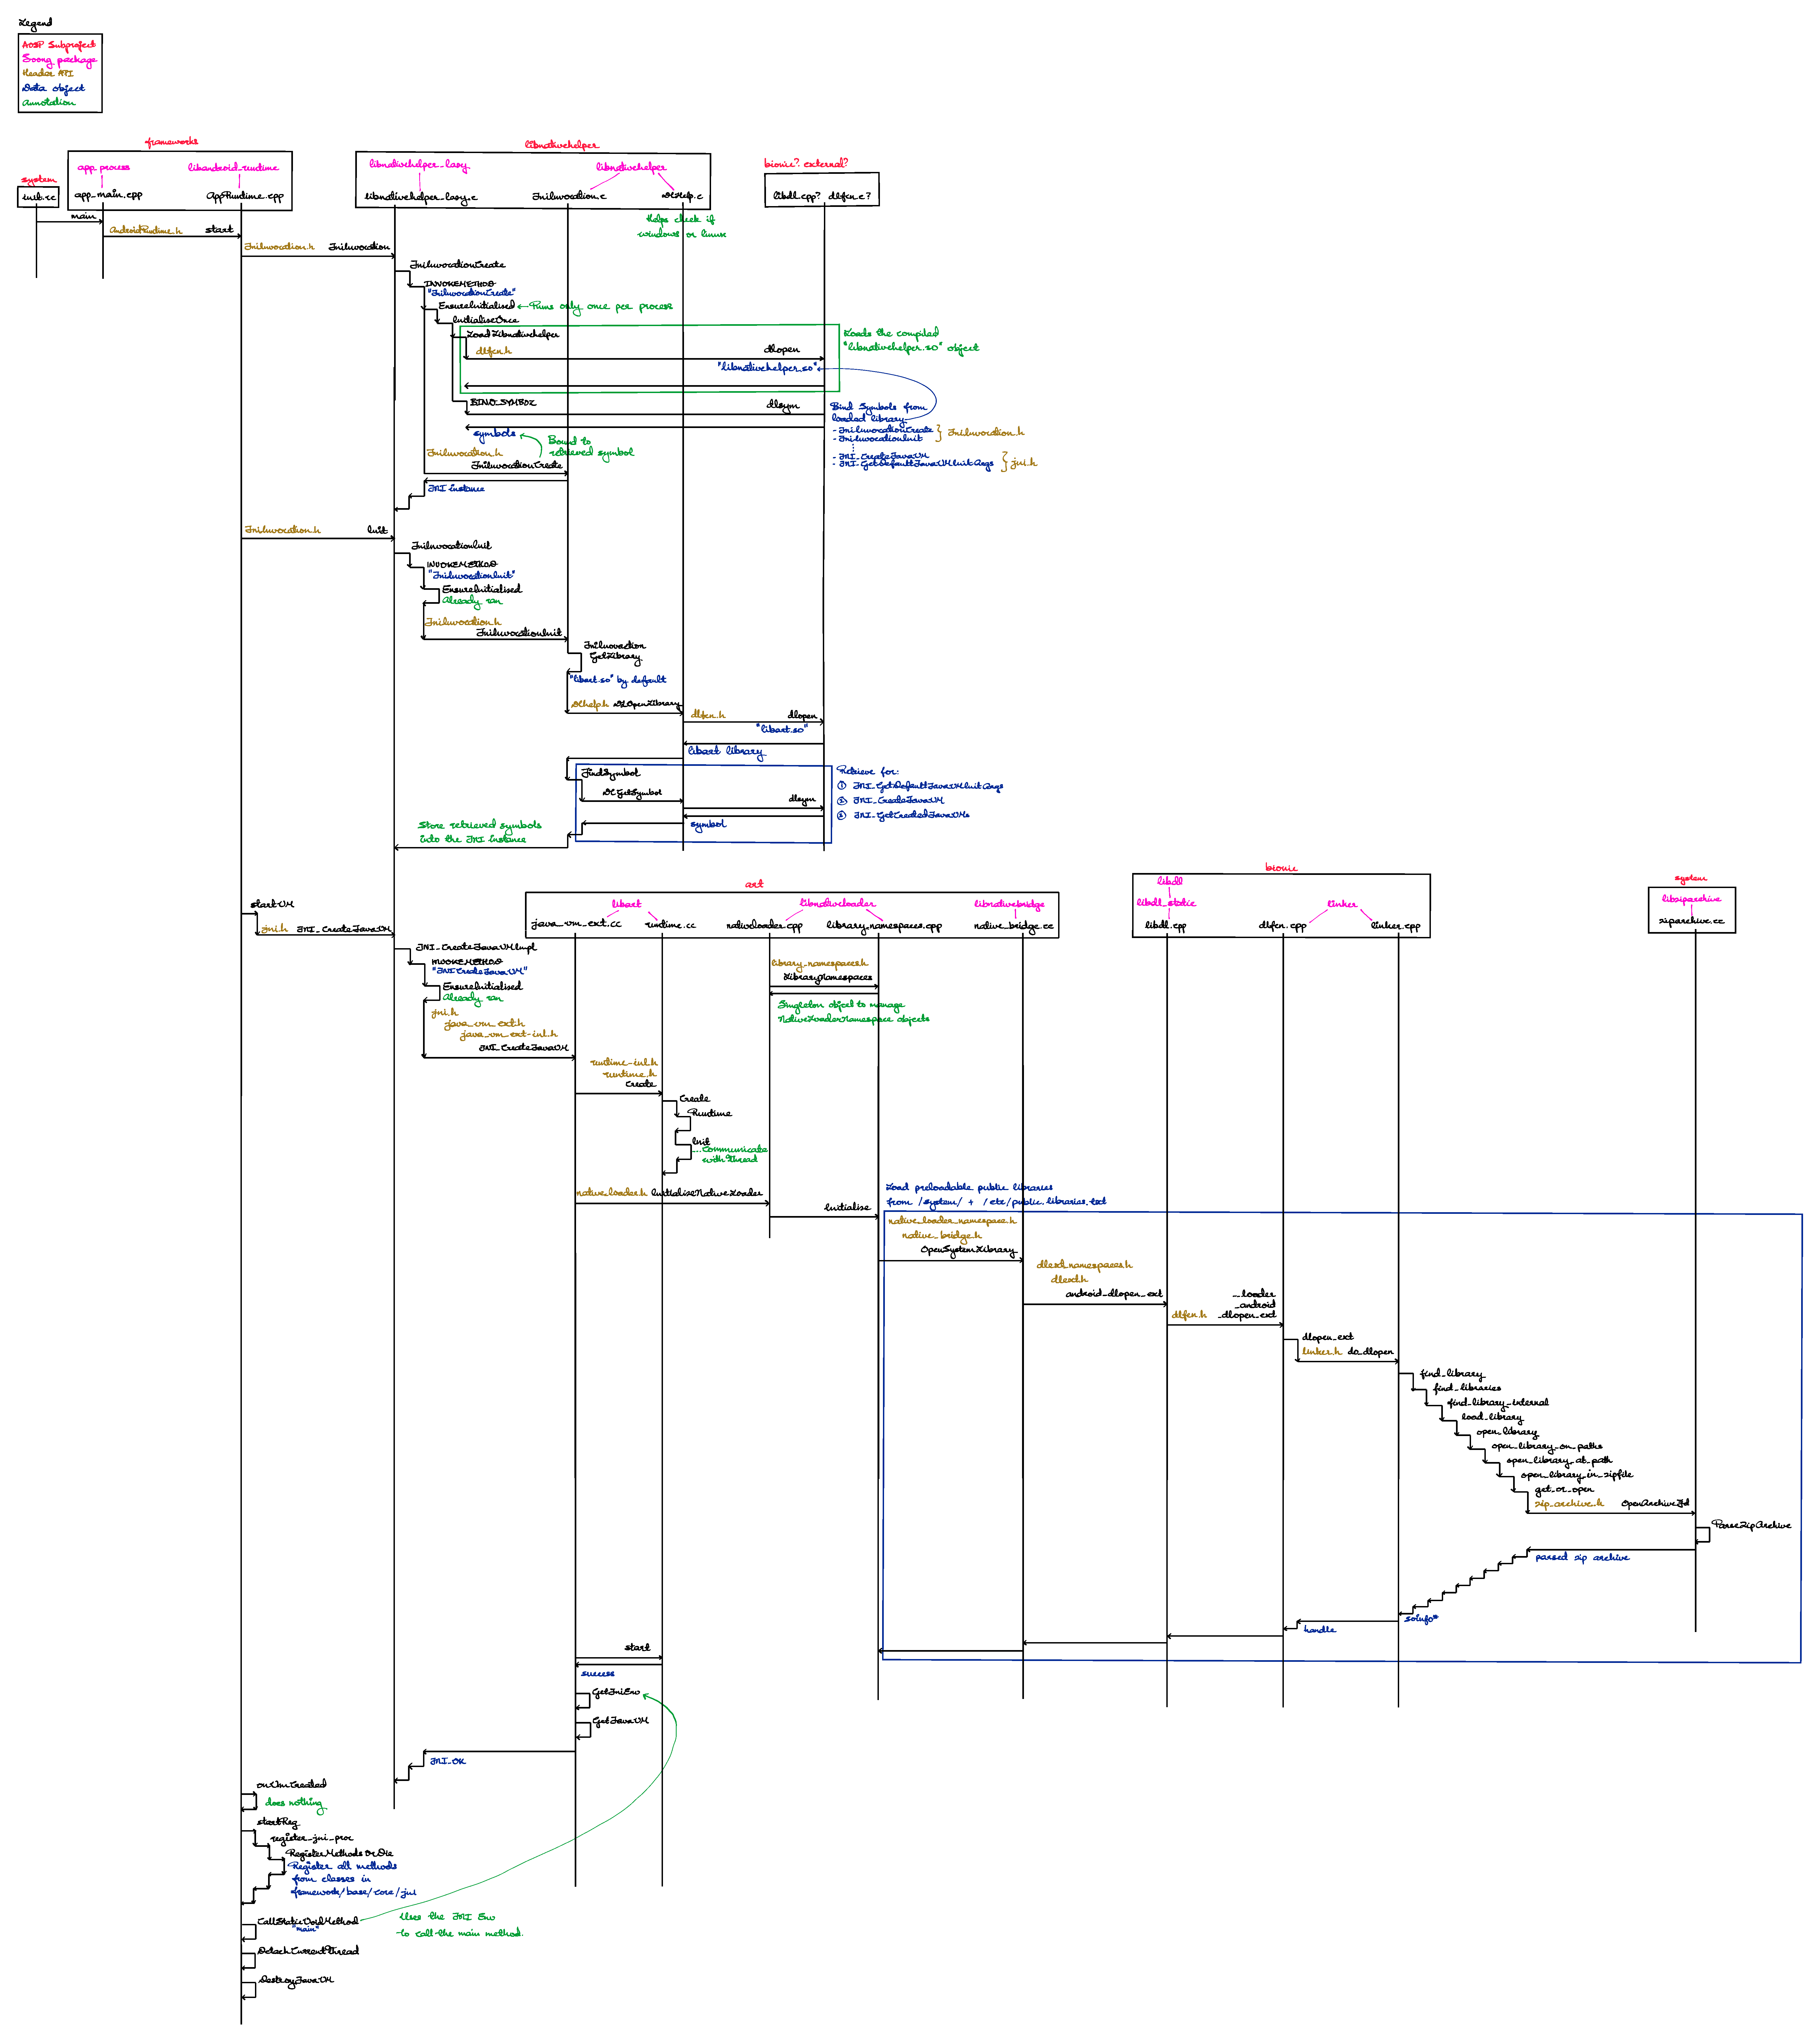
\includepdf[pages=-, scale=.95,pagecommand={}]{entries/2024/01/01/art.pdf}

% \begin{itemize}
% \item \textbf{Domain.} The context of the process that is acting upon something.
% \item \textbf{Type.} The context of the resource on which the process is acting.
% \item \textbf{Class.} The object class of the resource (e.g. \textit{file} or \textit{socket}).
% \item \textbf{Permissions.} The permissions that are allowed given the \textit{domain}, \textit{type} and \textit{class}.
% \end{itemize}

% SELinux rule syntax:
% \begin{lstlisting}
% allow <domain> <type>:<class> { <permissions> };
% \end{lstlisting}

% \subsubsection{Decoding Permission Denial Message}

% Message:
% \begin{lstlisting}
% type=AVC msg=audit(1363289005.532:184): avc:  denied  { read } for  pid=29199 comm="Trace" 
% name="online" dev="sysfs" ino=30 scontext=staff_u:staff_r:googletalk_plugin_t 
% tcontext=system_u:object_r:sysfs_t tclass=file
% \end{lstlisting}

% \begin{longtable}{p{.15\linewidth}p{.15\linewidth}p{.65\linewidth}} 
% \toprule
% Log part & Name & Description \\
% \midrule
% \endhead

% \texttt{type=AVC}
% &Log type
% &Only in the \texttt{audit.log} file; it informs the user what kind of audit log type this is. 
% \\

% \texttt{msg=audit(1363289005.532:184)}
% &Timestamp
% &Timestamp in seconds since epoch, meaning the number of seconds since January 1st, 1970. You can convert this to a more human readable format using date -d @ followed by the number, like so: \texttt{date -d @1363292159.532}.
% \\

% \texttt{avc:}
% &Log type (again)
% &
% \\

% \texttt{ino=30}
% &inode number
% &The inode number of the target file. In this case, since we know it is on the \texttt{sysfs} file system, we can look for this file using: \texttt{find /sys -xdev -inum 30}
% \\

% \texttt{scontent=staff\_u:staff\_r:googletalk\_plugin\_t}
% &Source context
% &The security context of the process (the domain)
% \\

% \texttt{tcontext=system\_u:object\_r:sysfs\_t}
% &Target context
% &The security context of the target resource (in this case the file)
% \\

% \texttt{tclass=file}
% &Target class
% &The class of the target.
% \\

% \midrule
% \caption{Permission Denied Syntax} 
% \label{tab:permissiondeniedsyntax}
% \end{longtable}


% \subsubsection{SELinux Architecture}

% SELinux consists of four main components: object managers (OM), access vector cache (AVC), security server, and security policy as show below:
% \begin{figure}[H]
%     \centering
%     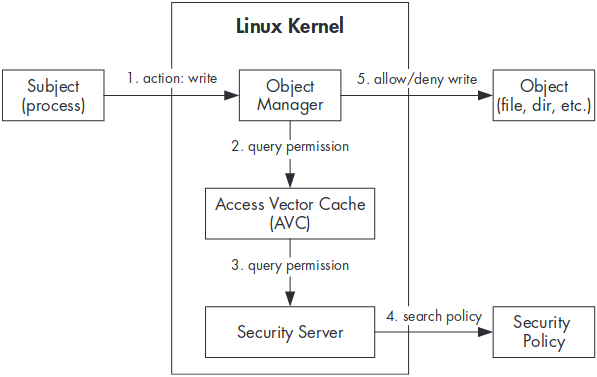
\includegraphics[width=.85\linewidth]{entries/2023/12/10/selinux.png}
%     \caption{SELinux Components}
%     \label{fig:selinux}
% \end{figure}
